\begin{oddBlock}{Box Passing (10 min)}

\begin{minipage}[t]{\linewidth}
    \centering
    
    \begin{minipage}{.3\linewidth} % Left column and width
        %\begin{figure}
            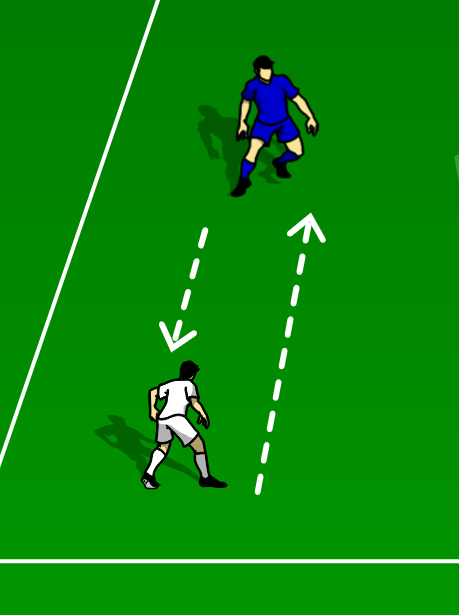
\includegraphics[width=.6\textwidth]{../img/Trimmed/Lane_Passing}
        %    \caption{Drill: 4 Person Passing}
        %\end{figure}
    \end{minipage}
    \hspace{0.05\linewidth}
    \begin{minipage}{.6\linewidth} % Left column and width
        \textbf{Drill Description:}

        \begin{enumerate}
        \setlength{\itemsep}{0pt}
        \setlength{\parskip}{0pt}
        \setlength{\parsep}{0pt}
        \item Two players stand in a 2 yard square box.  Boxes should be spaced about 5 yards apart.
        \item Players pass the ball to their partner in the 2 yard box.
        \item The partner tries to trap the ball within the box and pass it back.
        \end{enumerate}

        \textbf{Coaching Points:}
        \begin{itemize}
        \setlength{\itemsep}{0pt}
        \setlength{\parskip}{0pt}
        \setlength{\parsep}{0pt}
        \item Focus on passing accurately with pace.
        \item The goal is to trap the pass using a single touch.
        \end{itemize}

    \end{minipage}
\end{minipage}

\end{oddBlock}